\documentclass{article}
\usepackage{amsmath}
\usepackage{amssymb}
\usepackage{ctex}
\usepackage[margin=2cm]{geometry} % 设置较窄的边距使文档宽一些
\usepackage{multirow} % 支持表格中的多行单元格
\usepackage{graphicx} % 用于插入图片
\title{\heiti\zihao{2} 一阶 RC 电路过渡过程的研究}
\author{\songti  author  Student ID  \\
课程号  XXXXXX.01 }
\date{2024.4.22}
\begin{document}
    \maketitle
    
\begin{abstract}
    本实验旨在研究一阶 RC 电路的过渡过程。通过对 RC 电路的实验,我们可以深入了解电容器和电阻器在电路中的作用,以及它们如何影响电流和电压的变化。实验中,我们将测量电容器充放电过程中的电压和电流,并绘制相应的曲线图。通过对实验数据的分析,我们可以验证 RC 电路的理论模型,并计算出电路的时间常数。此外,我们还将探讨 RC 电路在实际应用中的重要性,如滤波器和延时电路等。
    通过本实验,我们不仅可以加深对 RC 电路的理解,还可以提高数据处理和分析的能力。这些技能在电子工程和物理学研究中都是非常重要的。我们希望通过本实验,能够更好地掌握一阶 RC 电路的基本原理和应用,为今后的学习和研究打下坚实的基础。
    
    \noindent{\textbf{关键词:} 一阶 RC 电路;过渡过程;时间常数;数据分析;实验研究}
\end{abstract}


\section{引言}
\label{sec:introduction}
    一阶 RC 电路是电子学中最基本的电路之一,由一个电阻器和一个电容器串联或并联组成。它们在电路中起着重要的作用,尤其是在信号处理和滤波等应用中。了解一阶 RC 电路的过渡过程对于掌握更复杂的电路设计和分析至关重要。
    
    在本实验中,我们将研究一阶 RC 电路的充放电过程,测量电容器两端的电压和电流,并绘制相应的曲线图。通过对实验数据的分析,我们可以验证 RC 电路的理论模型,并计算出电路的时间常数。此外,我们还将探讨 RC 电路在实际应用中的重要性,如滤波器和延时电路等。
    
\section{实验目的}
\begin{enumerate}
    \item 研究一阶 RC 电路的时域响应。
    \item 学会用示波器观察电路的时域响应。 
    \item 学习用示波器观察波形变换电路的波形及时间常数对它们的影响。
    \item 进一步了解微分电路和积分电路。 
\end{enumerate}

\section{实验原理}
1.动态网络的过渡过程是十分短暂的单次变化过程。要用普通示波器观察过渡过程和测量有关的参数,就必须使这种单次变化的过程重复出现。为此,我们利用信号发生器输出的方波来模拟阶跃激励信号,即利用方波输出的上升沿作为零状态响应的正阶跃激励信号;利用方波的下降沿作为零输入响应的负阶跃激励信号。只要选择方波的重复周期远大于电路的时间常数 $\tau$ ,那么电路在这样的方波序列脉冲信号的激励下,它的响应就和直流电接通与断开的过渡过程是基本相同的。

2.图 1(b)所示的 RC 一阶电路的零输入响应和零状态响应分别按指数规律衰减和增长,其变化的快慢决定于电路的时间常数 $\tau$ 。

3.时间常数 $\tau$ 的测定方法:
用示波器测量零输入响应的波形如图 1(a)所示。
根据一阶微分方程的求解得知 $\mathrm{u}_{\mathrm{c}}=\mathrm{U}_{\mathrm{m}} \mathrm{e}^{-t / R C}=U_m \mathrm{e}^{-\mathrm{t} /{ }^\tau}$ 。当 $\mathrm{t}=\tau$ 时, $\mathrm{Uc}(\tau)=0.368 \mathrm{U}_{\mathrm{m}}$ 。此时所对应的时间就等于 $\tau$ 。亦可用零状态响应波形增加到 $0.632 \mathrm{U}_{\mathrm{m}}$ 所对应的时间测得,如图 1(c)所示。

\begin{figure}[h]
    \centering
    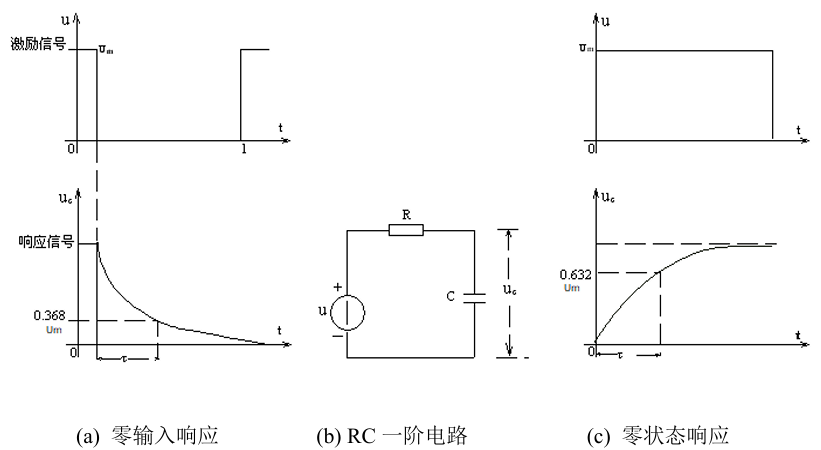
\includegraphics[width=0.8\textwidth]{img1.png}
    \caption{RC 电路的零输入响应和零状态响应}
    \label{fig:rc_circuit}
\end{figure}

4. 微分电路和积分电路是 RC 一阶电路中较典型的电路,它对电路元件参数和输入信号的
周期有着特定的要求。一个简单的 RC 串联电路,在方波序列脉冲的重复激励下,当满足 
$\tau=RC<<\frac{T}{2}$ 
时(T 为方波脉冲的重复周期),且由 R 两端的电压作为响应输出,则该电路就是一
个微分电路。因为此时电路的输出信号电压与输入信号电压的微分成正比。如图 3-2(a) 所示。利
用微分电路可以将方波转变成尖脉冲。
\begin{figure}[h]
    \centering
    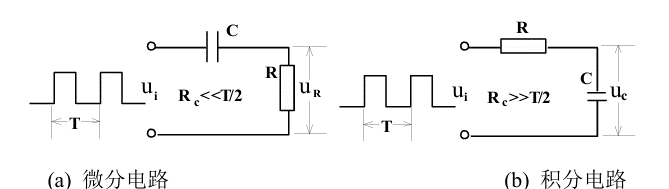
\includegraphics[width=0.8\textwidth]{img2.png}
    \caption{微分电路}
    \label{fig:diff_circuit}
\end{figure}

若将图 2(a)中的 $R$ 与 $C$ 位置调换一下,如图 2(b)所示,由 $C$ 两端的电压作为响应输出,
且当电路的参数满足 $\tau=\mathrm{RC} \gg \frac{T}{2}$ ,则该 RC 电路称为积分电路。
因为此时电路的输出信号电压与输入信号电压的积分成正比。利用积分电路可以将方波转变成三角波。

从输入输出波形来看,上述两个电路均起着波形变换的作用

输出取自电阻两端电压,构成微分电路。以输入方波信号为例,要使该电路能完美地实现微分,就要求时间常数 $\tau=R C \ll t_p$ ,其中 $t_p$ 是矩形脉冲宽度。由这个条件我们可以将电容电压 $u_c(t)$ 近似为电源电压 $u_s(t)$

$$
R C \ll t_p \text {, 则 } R C \ll T
$$


周期化作角频率,可得 $\frac{1}{\omega C} \gg R$

$$
\text { 所以,} u_c(t) \gg u_o(t), ~ u_c(t) \approx u_s(t)
$$


假设电压初始状态 $u_c\left(0_{-}\right)=0 V$ ,结合电容的电压与电流关系,可得电路输出是输入电压的微分:

$$
u_o(t)=i_c R=R C \frac{d u_c(t)}{d t} \approx \tau \frac{d u_s(t)}{d t}
$$

同样,积分电路也采用类似的分析方法。但不同于微分电路,时间常数 $\tau=R C \gg t_p$ 才能实现较好的积分效果。此时, $u_s(t) \approx u_R(t)$ 。

输出直接取自电容的电压,因此输出是输入电压的积分。

$$
u_o(t)=u_c(t)=\frac{1}{C} \int_0^t i_R(t) d t=\frac{1}{R C} \int_0^t u_R(t) d t \approx \frac{1}{\tau} \int_0^t U_s(t) d t
$$

\section{实验器材}
\label{sec:equipment}
    \begin{enumerate}
        \item 示波器
        \item 信号发生器
        \item 电阻: $R=100\Omega$, $R=1k\Omega$, $R=10k\Omega$, $R=1M\Omega$
        \item 电容: $C=0.1\mu F$, $C=0.01\mu F$, $C=6800 p F$, $C=1000 p F$
        \item 连接线若干
    \end{enumerate} 

\begin{figure}[h]
    \centering
    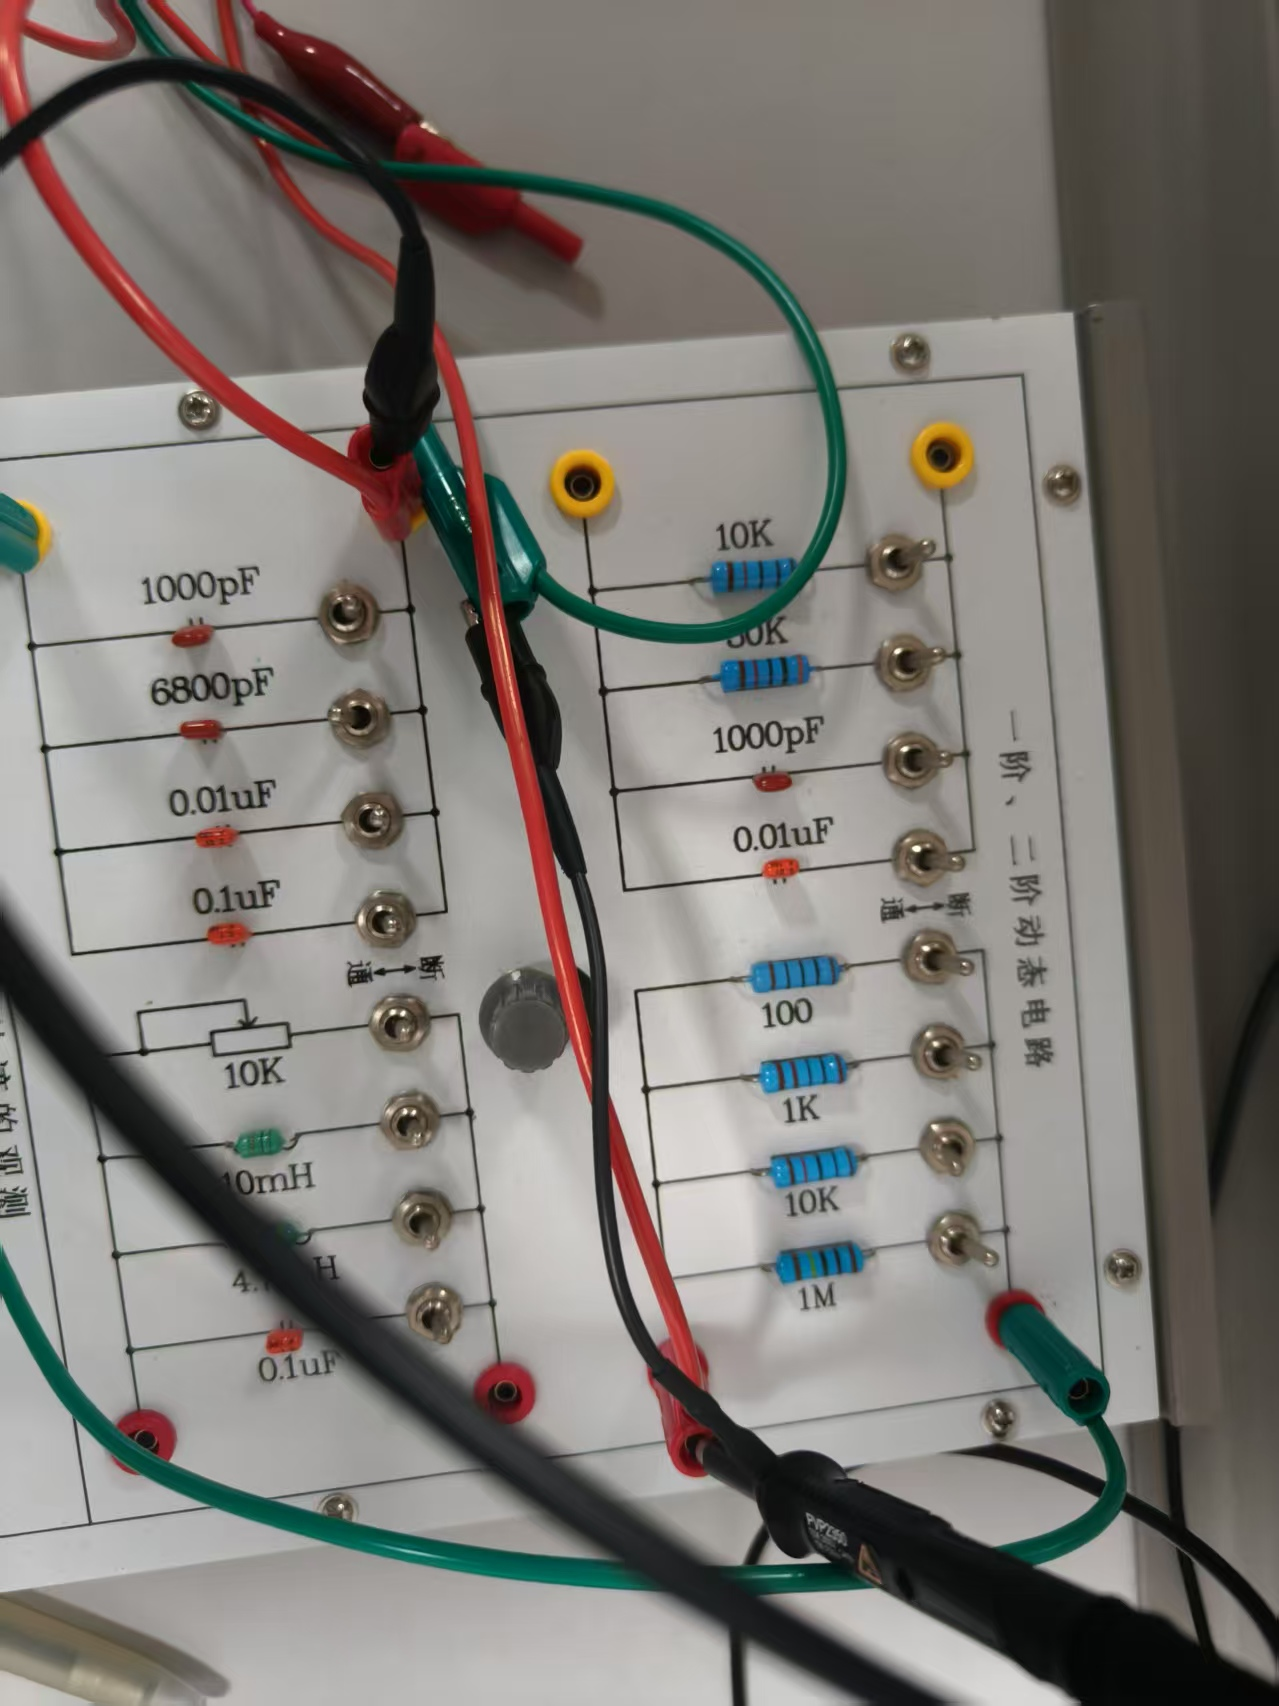
\includegraphics[width=0.4\textwidth]{实验器材.jpg}
    \caption{HE-14 动态电路实验板}
    \label{fig:equipment}
\end{figure}


\section{实验步骤}

\subsection{RC 电路积分过程}
(1)从电路板上选 $\mathrm{R}=10 \mathrm{~K} \Omega, \mathrm{C}=1000 \mathrm{pF}$ 组成如图 2(b)所示的 RC 充放电电路。U 为信号发生器输出的 $\mathrm{U}_{\mathrm{P}-\mathrm{P}}=3 \mathrm{~V}, ~ \mathrm{f}=1 \mathrm{KHz}$ 的方波电压信号,并通过两根同轴电缆线,将激励源 u 和响应 $\mathrm{u}_{\mathrm{c}}$ 的信号分别连至示波器的两个输入口 $\mathrm{Y}_{\mathrm{A}}$ 和 $\mathrm{Y}_{\mathrm{B}}$ 。这时可在示波器的屏幕上观察到激励与响应的变化规律,请测算出时间常数 $\tau$ ,并用方格纸按 1:1 的比例描绘波形。

保持 $\mathrm{R}=10 \mathrm{~K} \Omega$ 不变,继续增大 C 之值,依次拨动 $\mathrm{C}=6800 \mathrm{pF}, ~ \mathrm{C}=0.01 \mu \mathrm{~F}, ~ \mathrm{C}=0.1 \mu \mathrm{~F}$ ,观察并描绘响应的波形,定性地观察对响应的影响。

(2)时间常数 $\tau$ 的测定方法(充放电达到稳态时):既可以利用充电过程,也可以利用放电过程 $\mathrm{Uc}(\mathrm{t})$ 的波形测量时间常数。可以首先用光标的幅度测量功能,移动两条水平光标找到 $\mathrm{Uc}(\tau)$点,然后再用光标的时间测量功能,移动两条垂直光标找到测时间常数的位置,读出 $\tau$ 值。 $\tau$ 的
测量值可以取充、放电过程测量值的平均值。 
\subsection{RC 电路微分过程}

令 $\mathrm{C}=0.01 \mu \mathrm{~F}, \mathrm{R}=100 \Omega$ ,组成如图 2(a)所示的微分电路。在同样的方波激励信号( $\mathrm{U}_{\mathrm{P}-\mathrm{P}}$ $=3 \mathrm{~V}, \mathrm{f}=1 \mathrm{KHz}$ )作用下,观测并描绘激励与响应的波形。

保持 $\mathrm{C}=0.01 \mu \mathrm{~F}$ 不变,继续增大 R 之值,依次拨动 $\mathrm{R}=1 \mathrm{~K} \Omega, ~ \mathrm{R}=10 \mathrm{~K} \Omega, ~ \mathrm{R}=1 \mathrm{M} \Omega$ ,定性地观察对响应的影响,并作记录。

\section{实验数据与分析}
\begin{table}[h]
    \centering
    \begin{tabular}{cc}
        % 左侧:积分电路
        \begin{tabular}{|c|c|c|}
            \hline
            \textbf{电容} & \textbf{电阻} & \textbf{时间常数} \\
            \hline
            $1000\,\mathrm{pF}$ & $10\,\mathrm{k}\Omega$ & $10\,\mu s$ \\
            \hline
            $6800\,\mathrm{pF}$ & $10\,\mathrm{k}\Omega$ & $68\,\mu s$ \\
            \hline
            $0.01\,\mu F$ & $10\,\mathrm{k}\Omega$ & $100\,\mu s$ \\
            \hline
            $0.1\,\mu F$ & $10\,\mathrm{k}\Omega$ & $1\,ms$ \\
            \hline
        \end{tabular}
        &
        % 右侧:微分电路
        \begin{tabular}{|c|c|c|}
            \hline
            \textbf{电容} & \textbf{电阻} & \textbf{时间常数} \\
            \hline
            $0.01\,\mu F$ & $100\,\Omega$ & $1\,\mu s$ \\
            \hline
            $0.01\,\mu F$ & $1\,\mathrm{k}\Omega$ & $10\,\mu s$ \\
            \hline
            $0.01\,\mu F$ & $10\,\mathrm{k}\Omega$ & $100\,\mu s$ \\
            \hline
            $0.01\,\mu F$ & $1\,\mathrm{M}\Omega$ & $10\,ms$ \\
            \hline
        \end{tabular}
    \end{tabular}
    \caption{积分电路与微分电路的时间常数}
    \label{tab:rc_compare}
\end{table}
\subsection{积分电路}
 图 4(a)  $\mathrm{R}=10 \mathrm{~K} \Omega, \mathrm{C}=0.1 \mu \mathrm{F}$满足最好,积分电路实现了方波到三角波的变换,T 越小于时间常数,三角波的线性度越好


\begin{figure}[h]
    \centering
    \begin{tabular}{cc}
        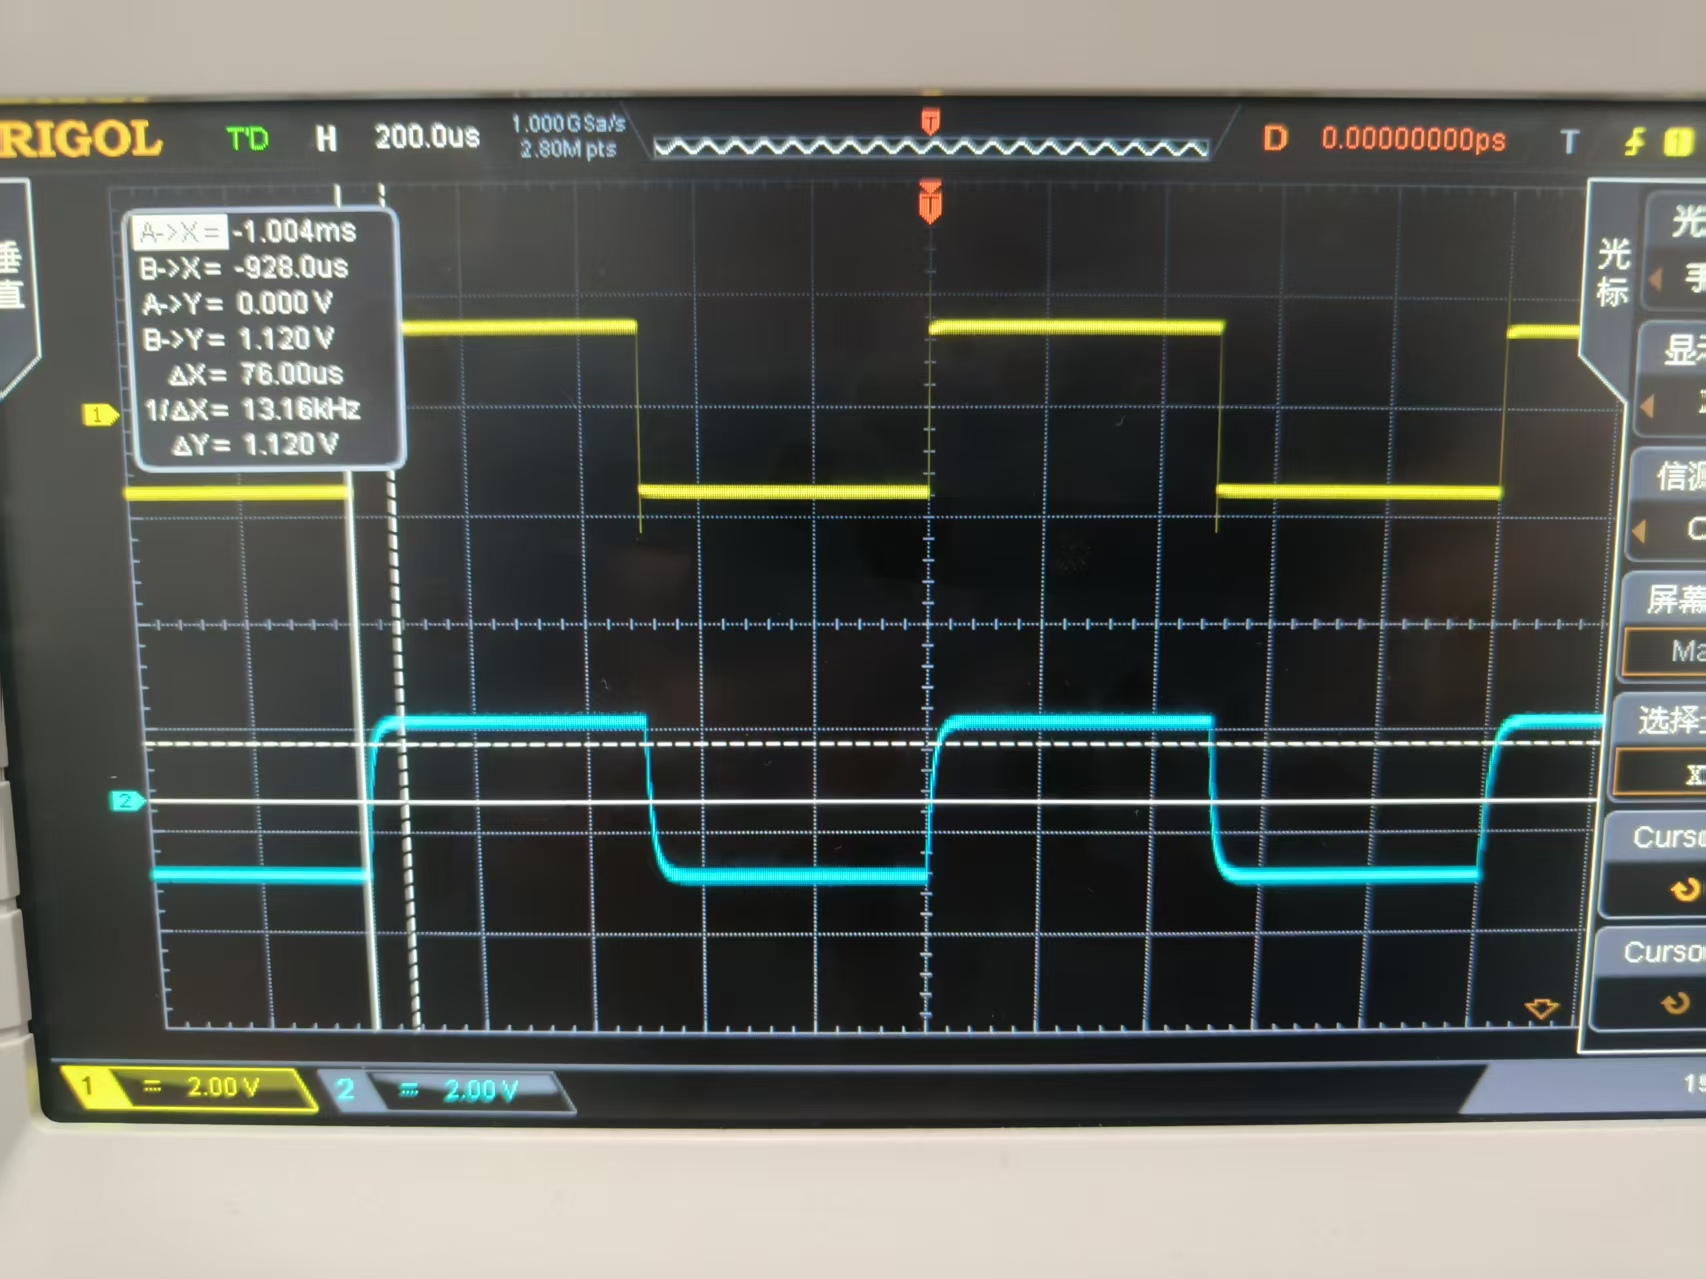
\includegraphics[width=0.35\textwidth]{0.1.jpg} &
        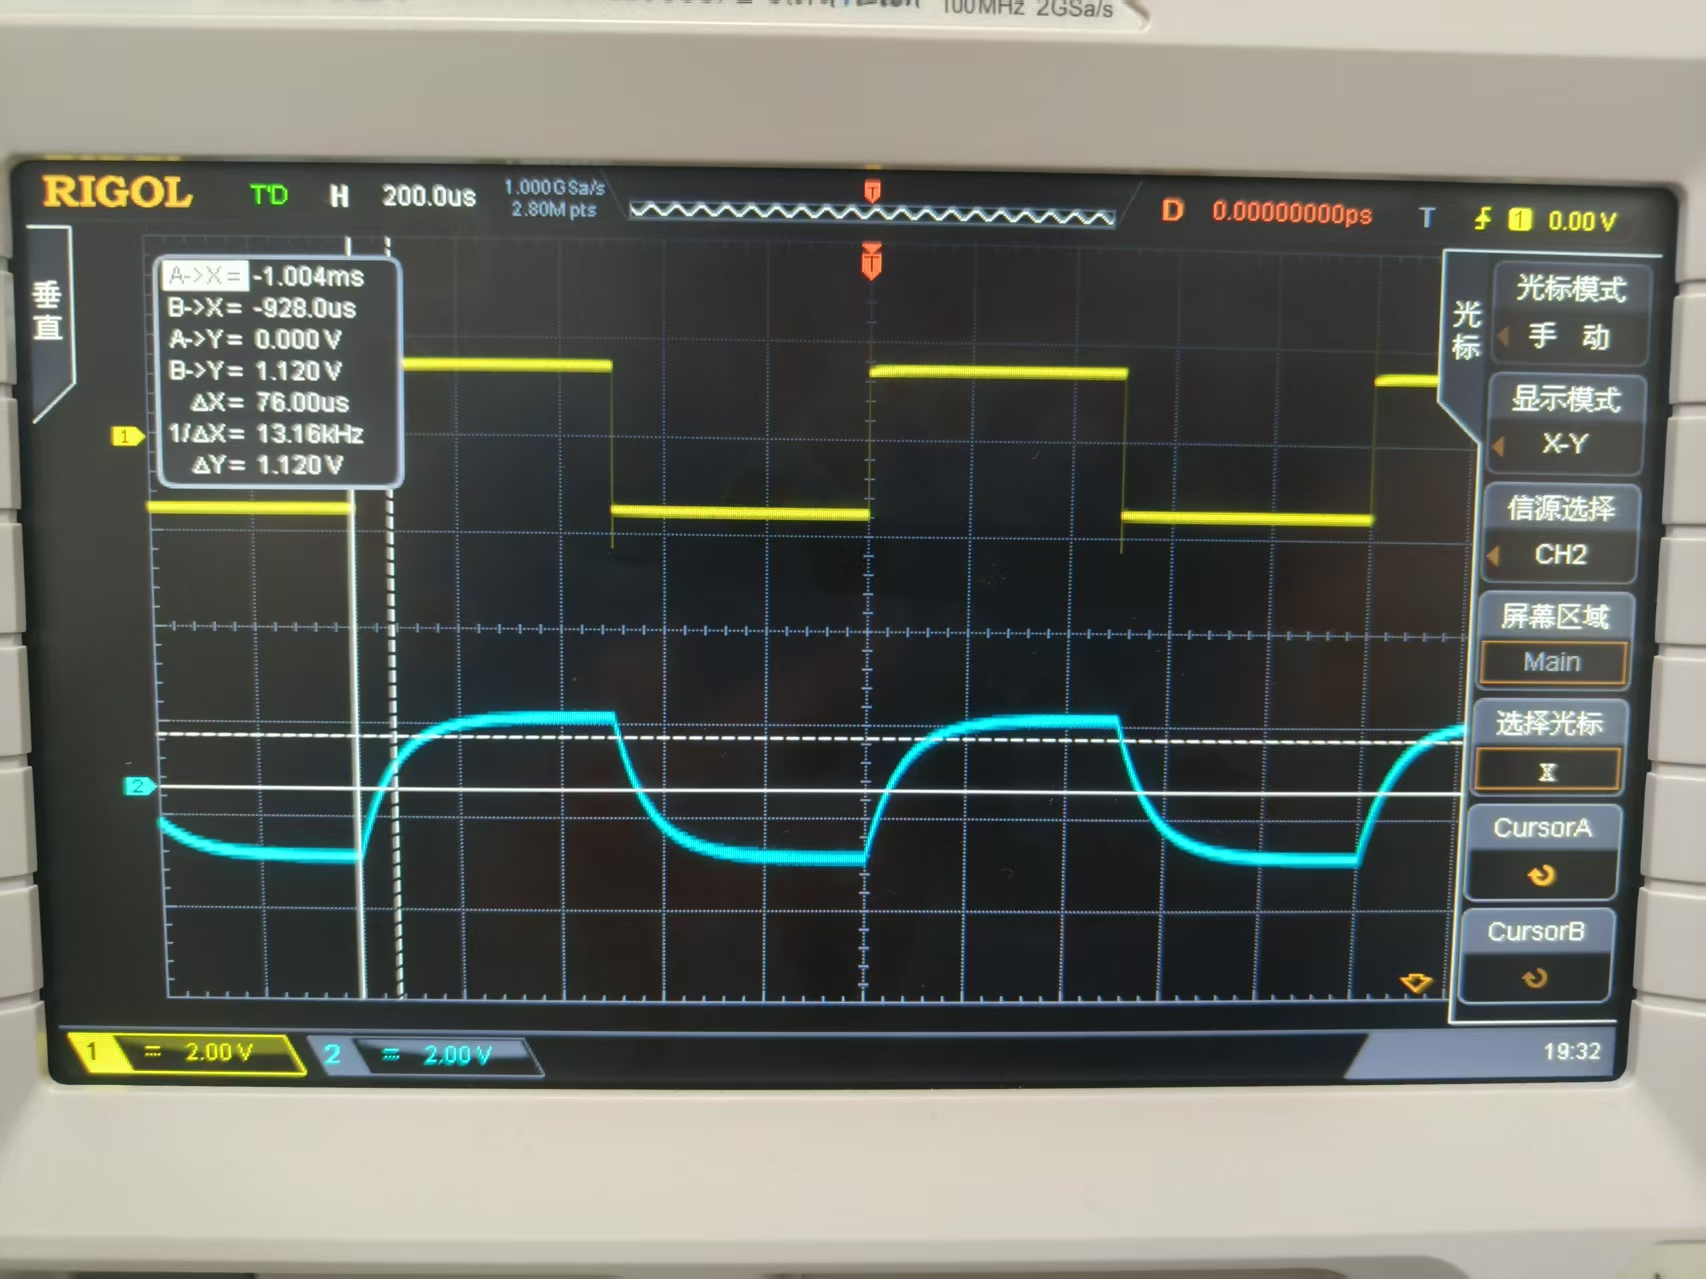
\includegraphics[width=0.35\textwidth]{0.01.jpg} \\
        (a) $\mathrm{C}=1000p \mathrm{~F}$& (b) $\mathrm{C}=6800p \mathrm{~F}$ \\
        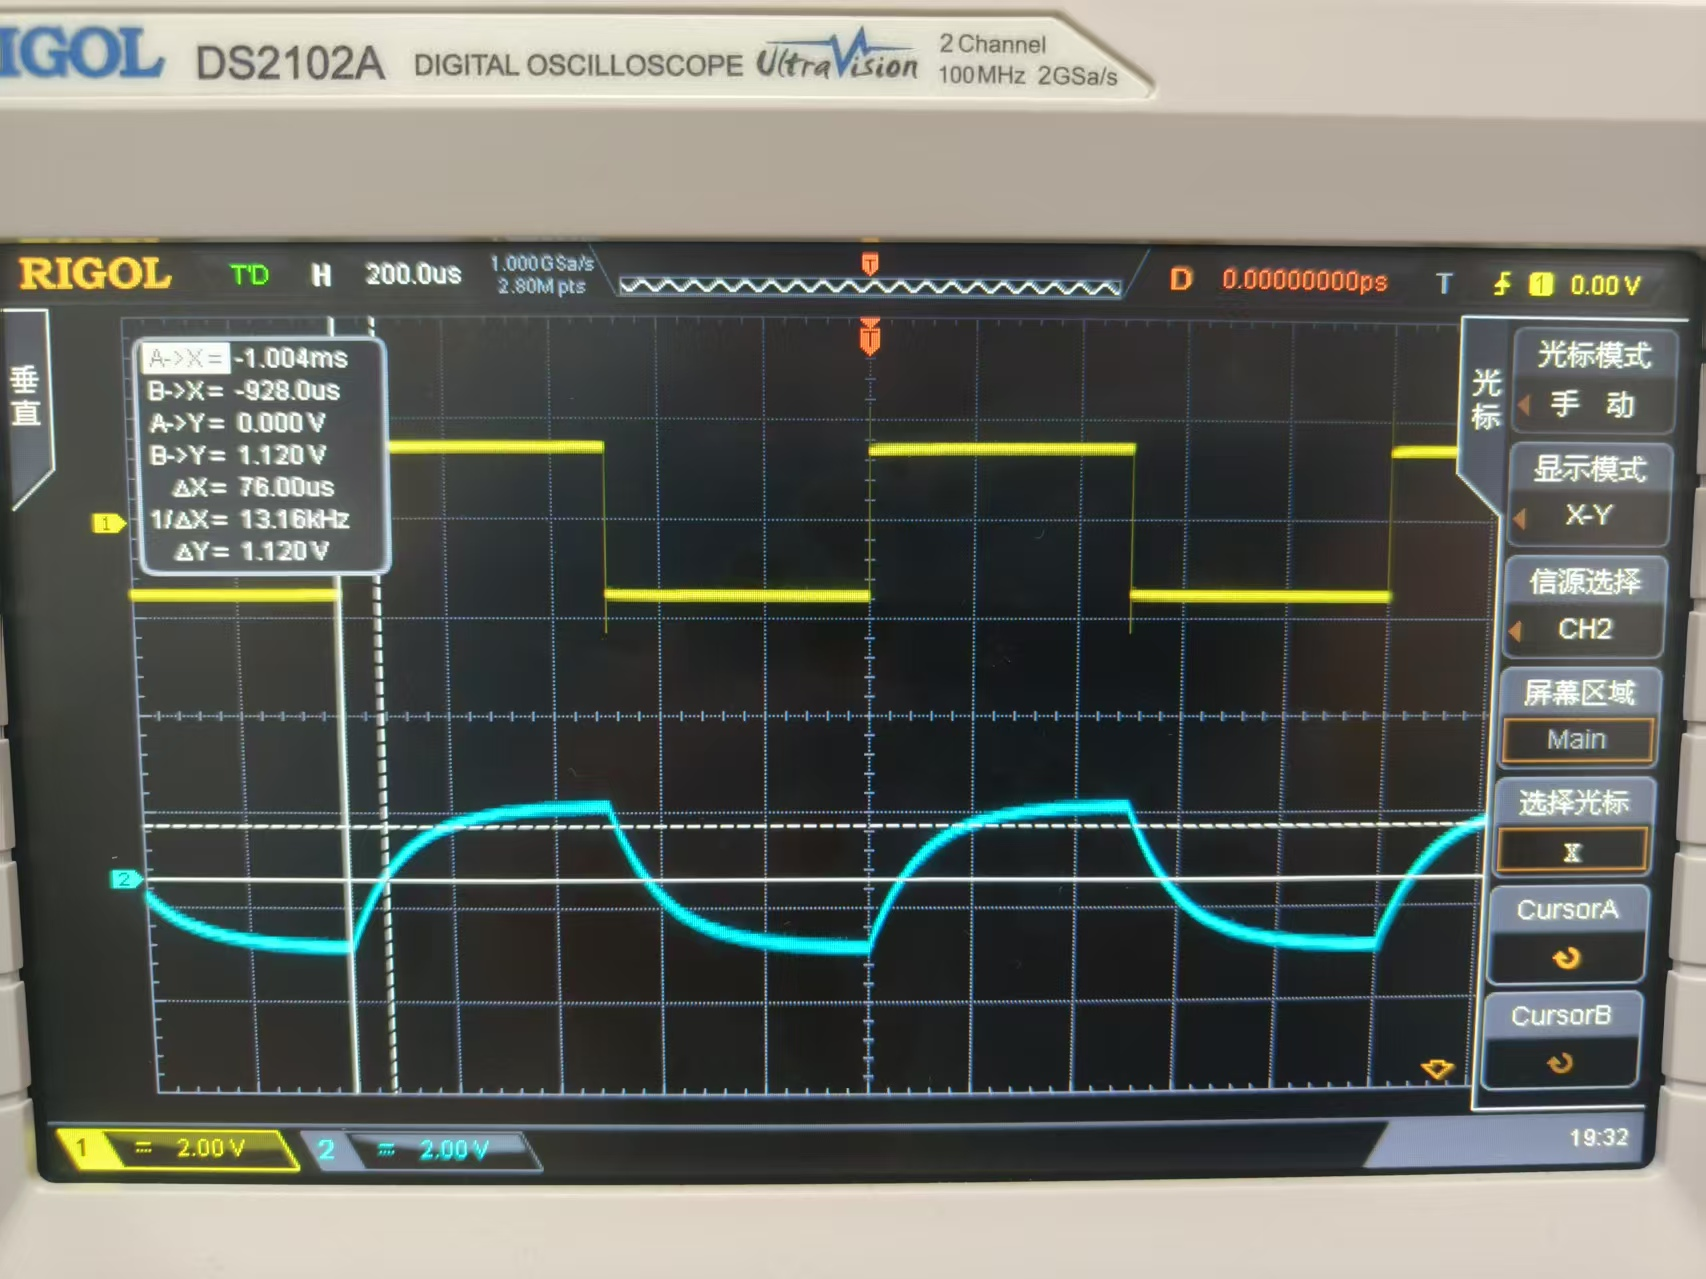
\includegraphics[width=0.35\textwidth]{6800.jpg} &
        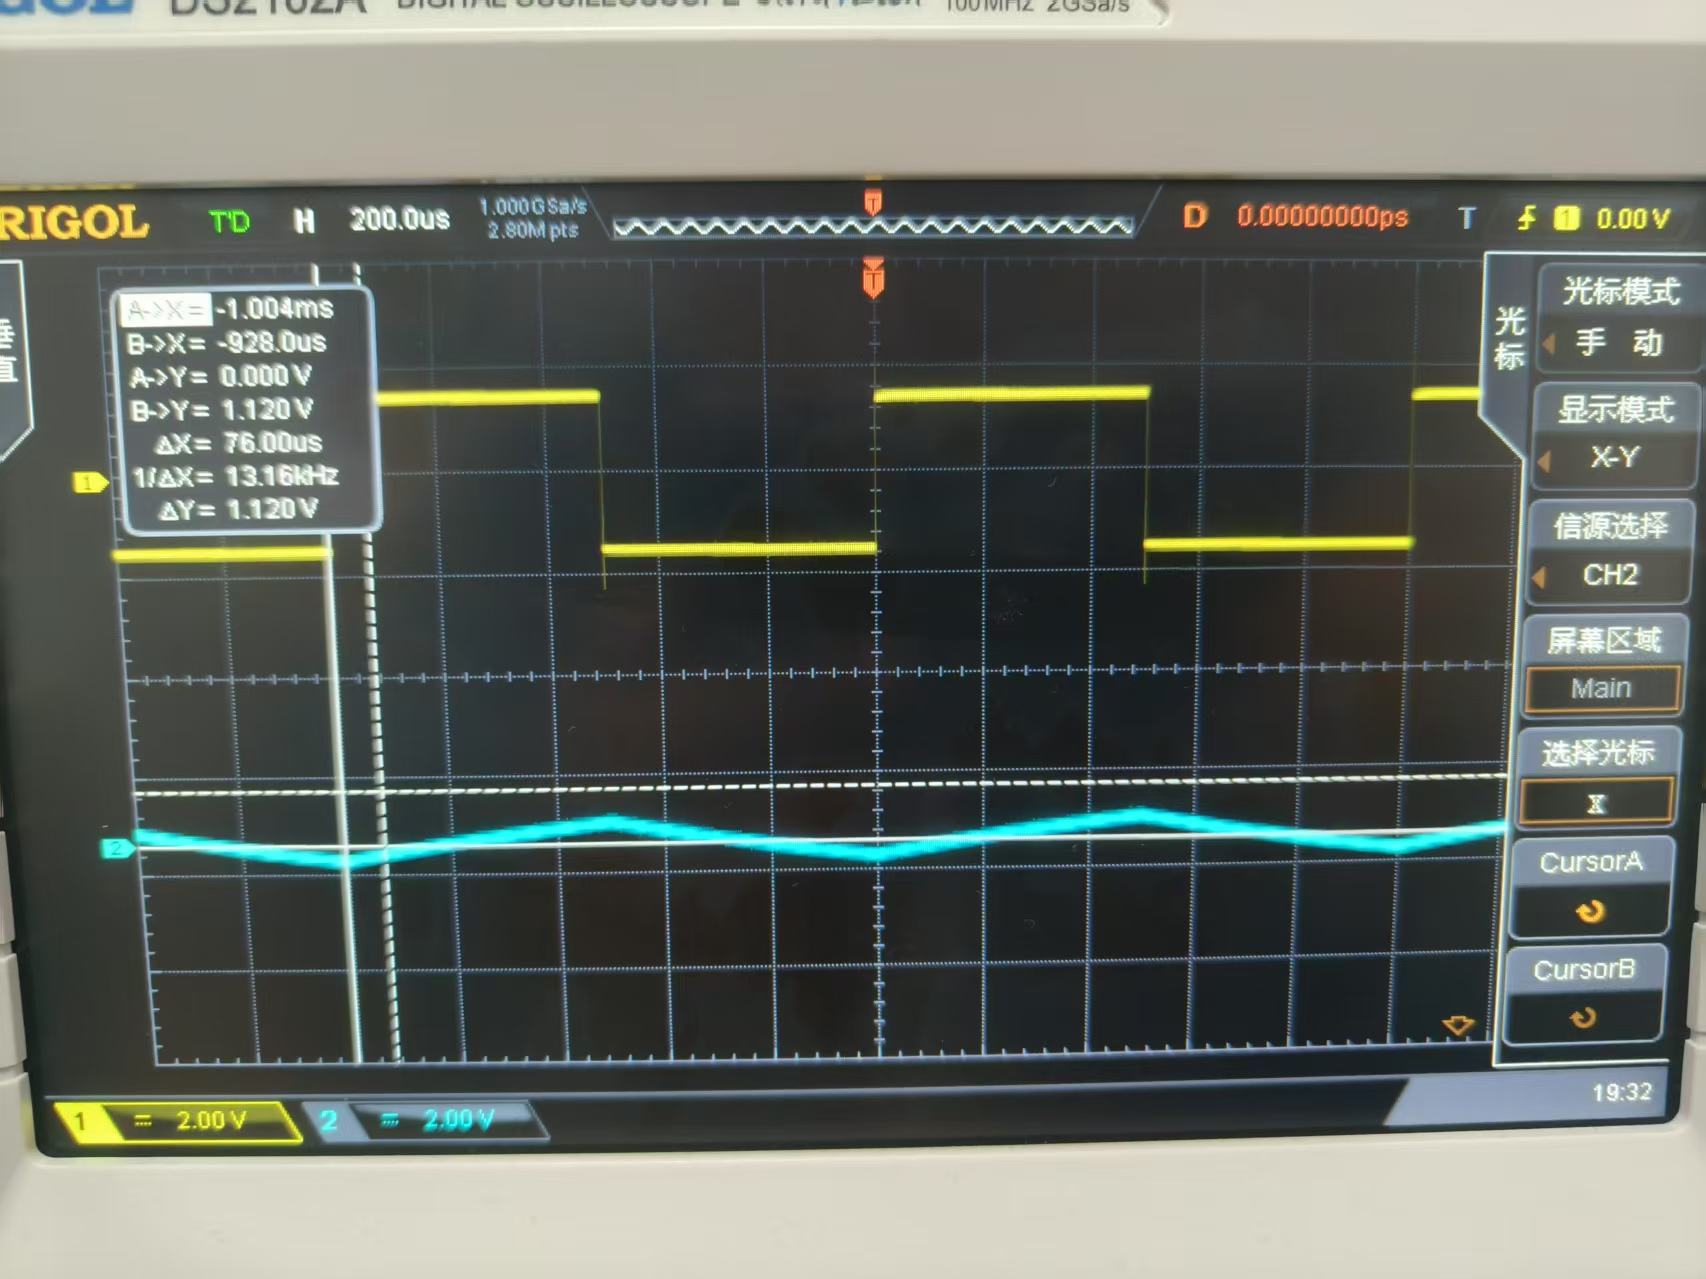
\includegraphics[width=0.35\textwidth]{1000.jpg} \\
        (c) $\mathrm{C}=0.01 \mu \mathrm{~F}$ & (d) $\mathrm{C}=0.1 \mu \mathrm{~F}$ \\
    \end{tabular}
    \caption{积分电路  $\mathrm{R}=10k \Omega $}
    \label{fig:grouped_images}
\end{figure}

\subsection{时间常数 $\tau$ 的测定}
图 5 所示 $\tau=68\mu s =RC$
\begin{figure}[h]
    \centering
    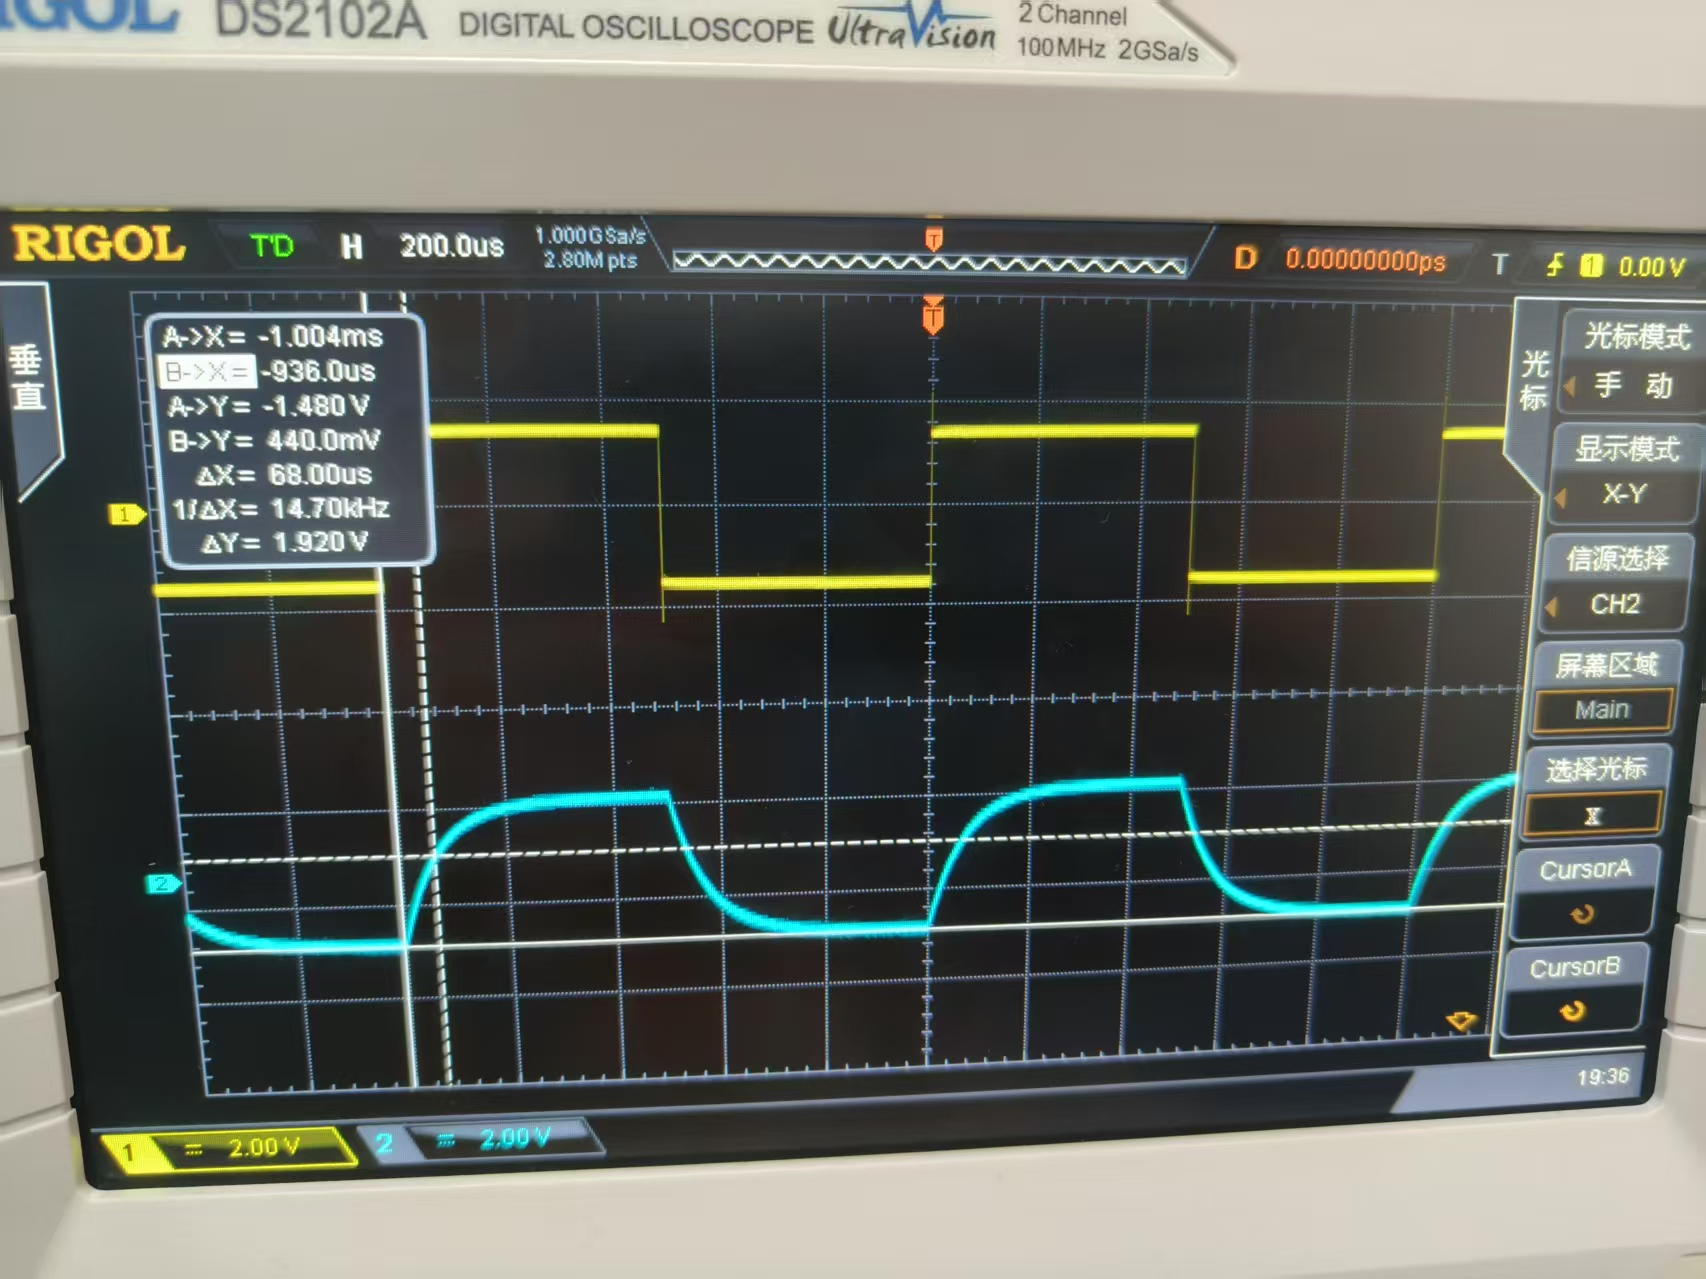
\includegraphics[width=0.8\textwidth]{RC.jpg}
    \caption{时间常数 $\tau$ 的测定}
    \label{fig:tau_measurement}
\end{figure}


\subsection{微分电路}
图 6(d) $\mathrm{R}=100 \Omega, \mathrm{C}=0.01 \mu \mathrm{F}$满足最好,RC 越小,尖脉冲波形越尖,反之则宽
\begin{figure}[h]
    \centering
    \begin{tabular}{cc}
        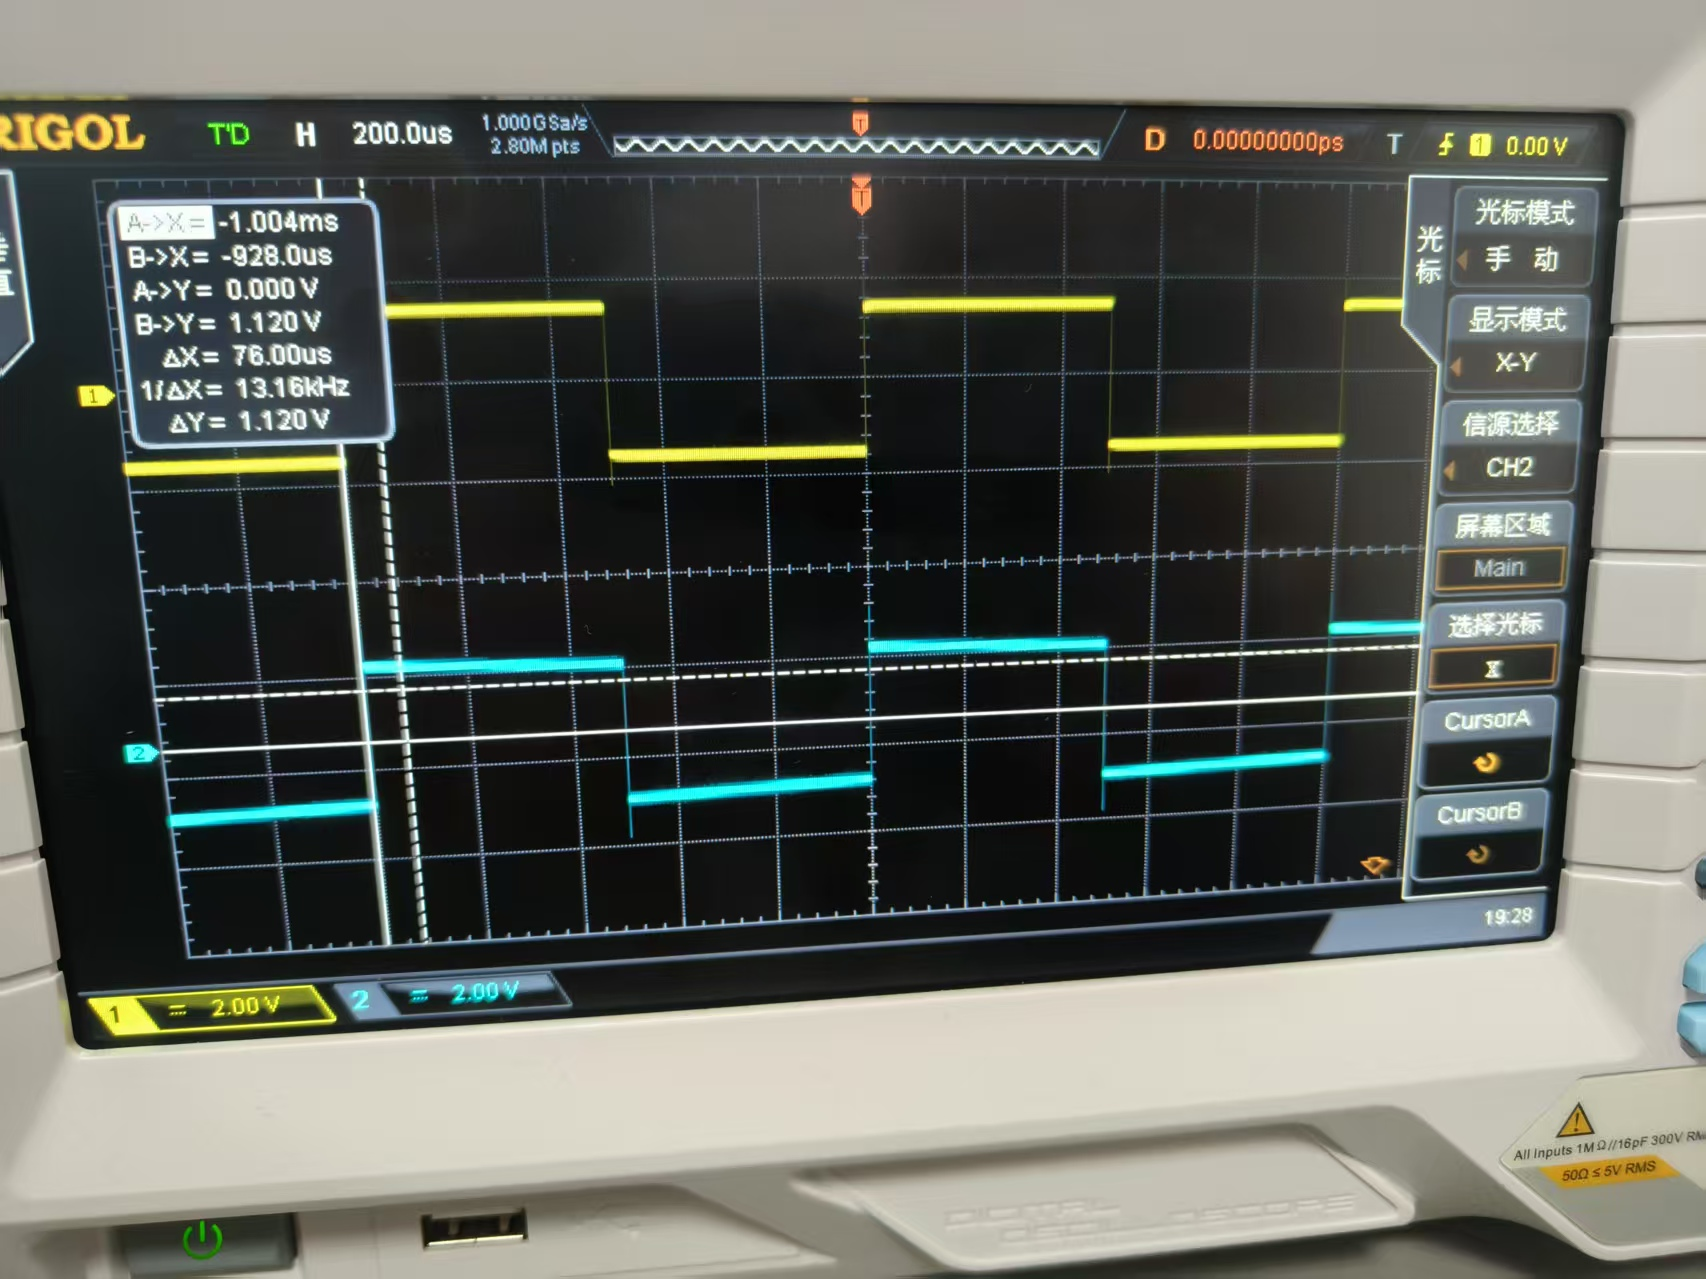
\includegraphics[width=0.35\textwidth]{1M.jpg} &
        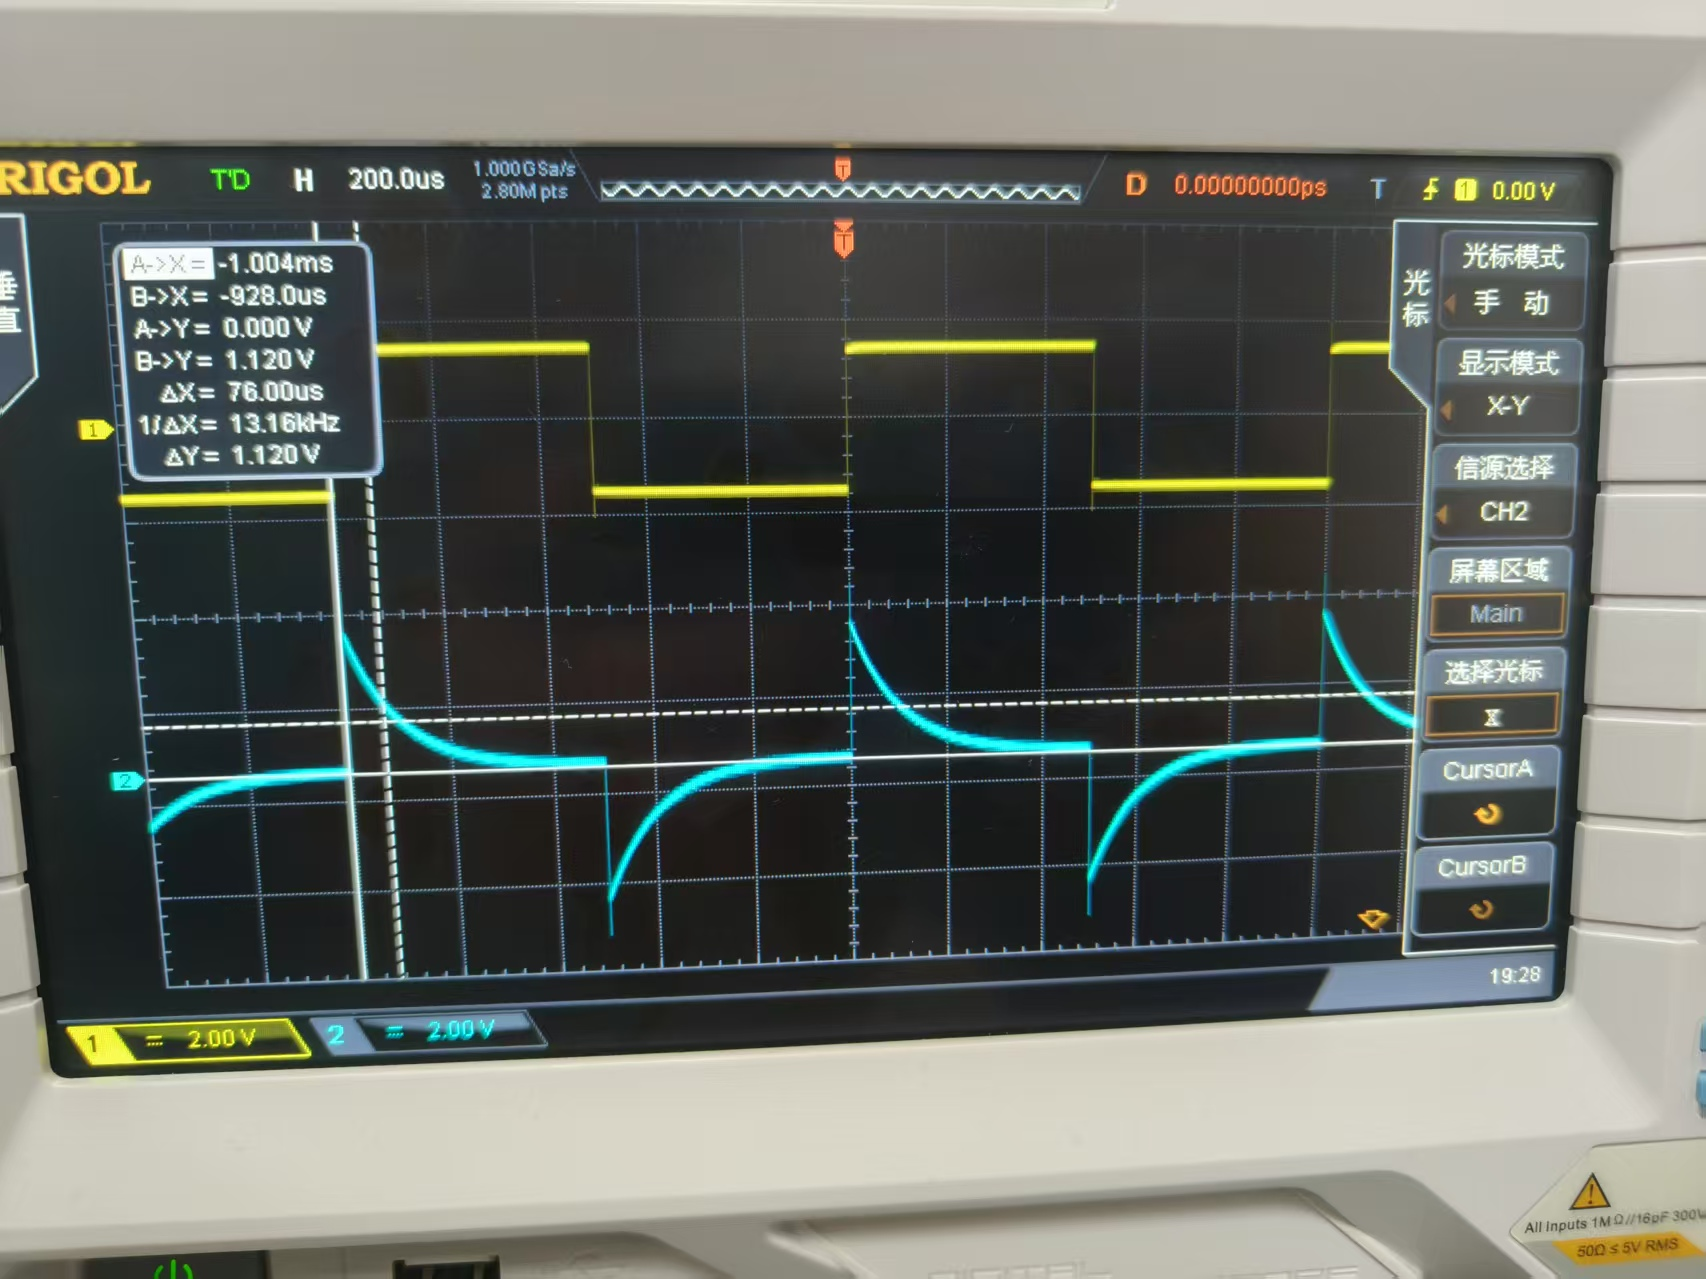
\includegraphics[width=0.35\textwidth]{10k.jpg} \\
        (a) $\mathrm{R}=1M \Omega $& (b) $\mathrm{R}=10k \Omega $ \\
        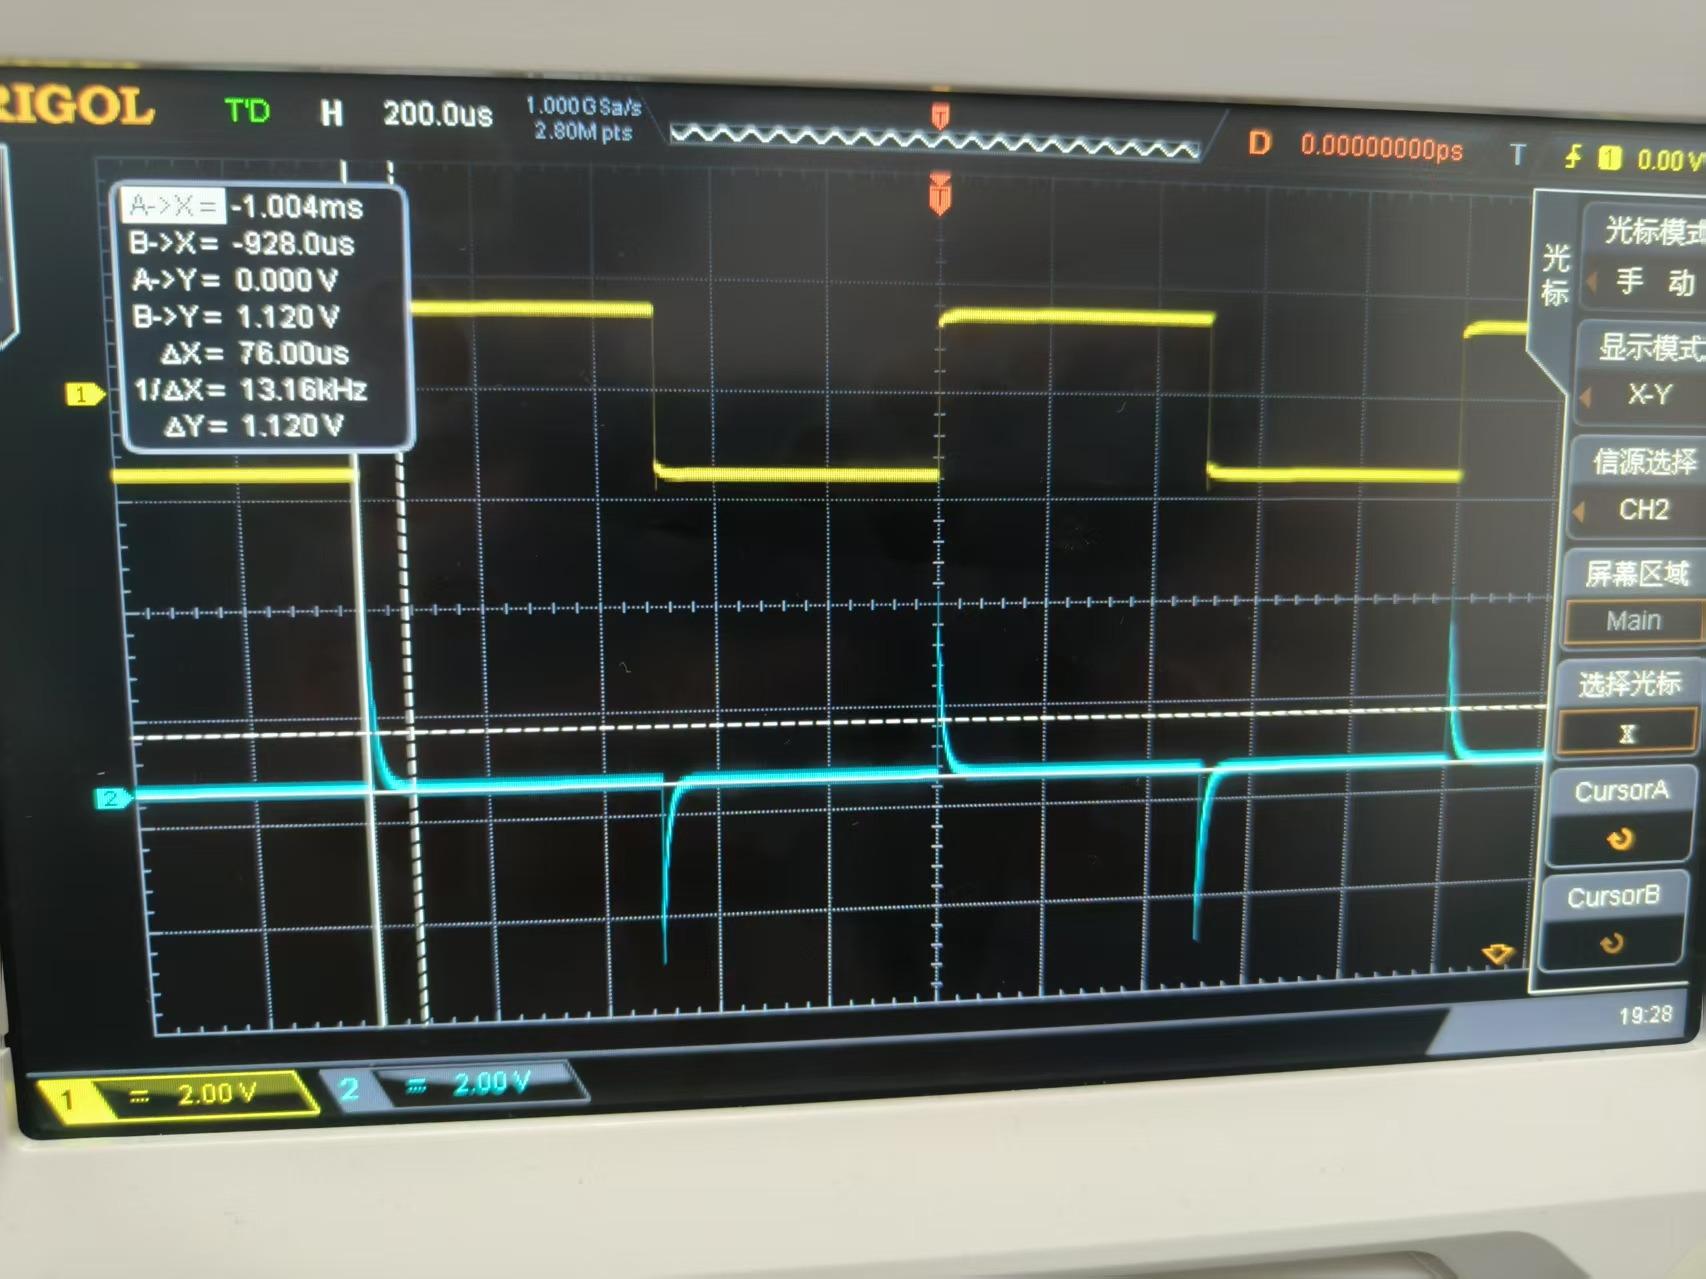
\includegraphics[width=0.35\textwidth]{1k.jpg} &
        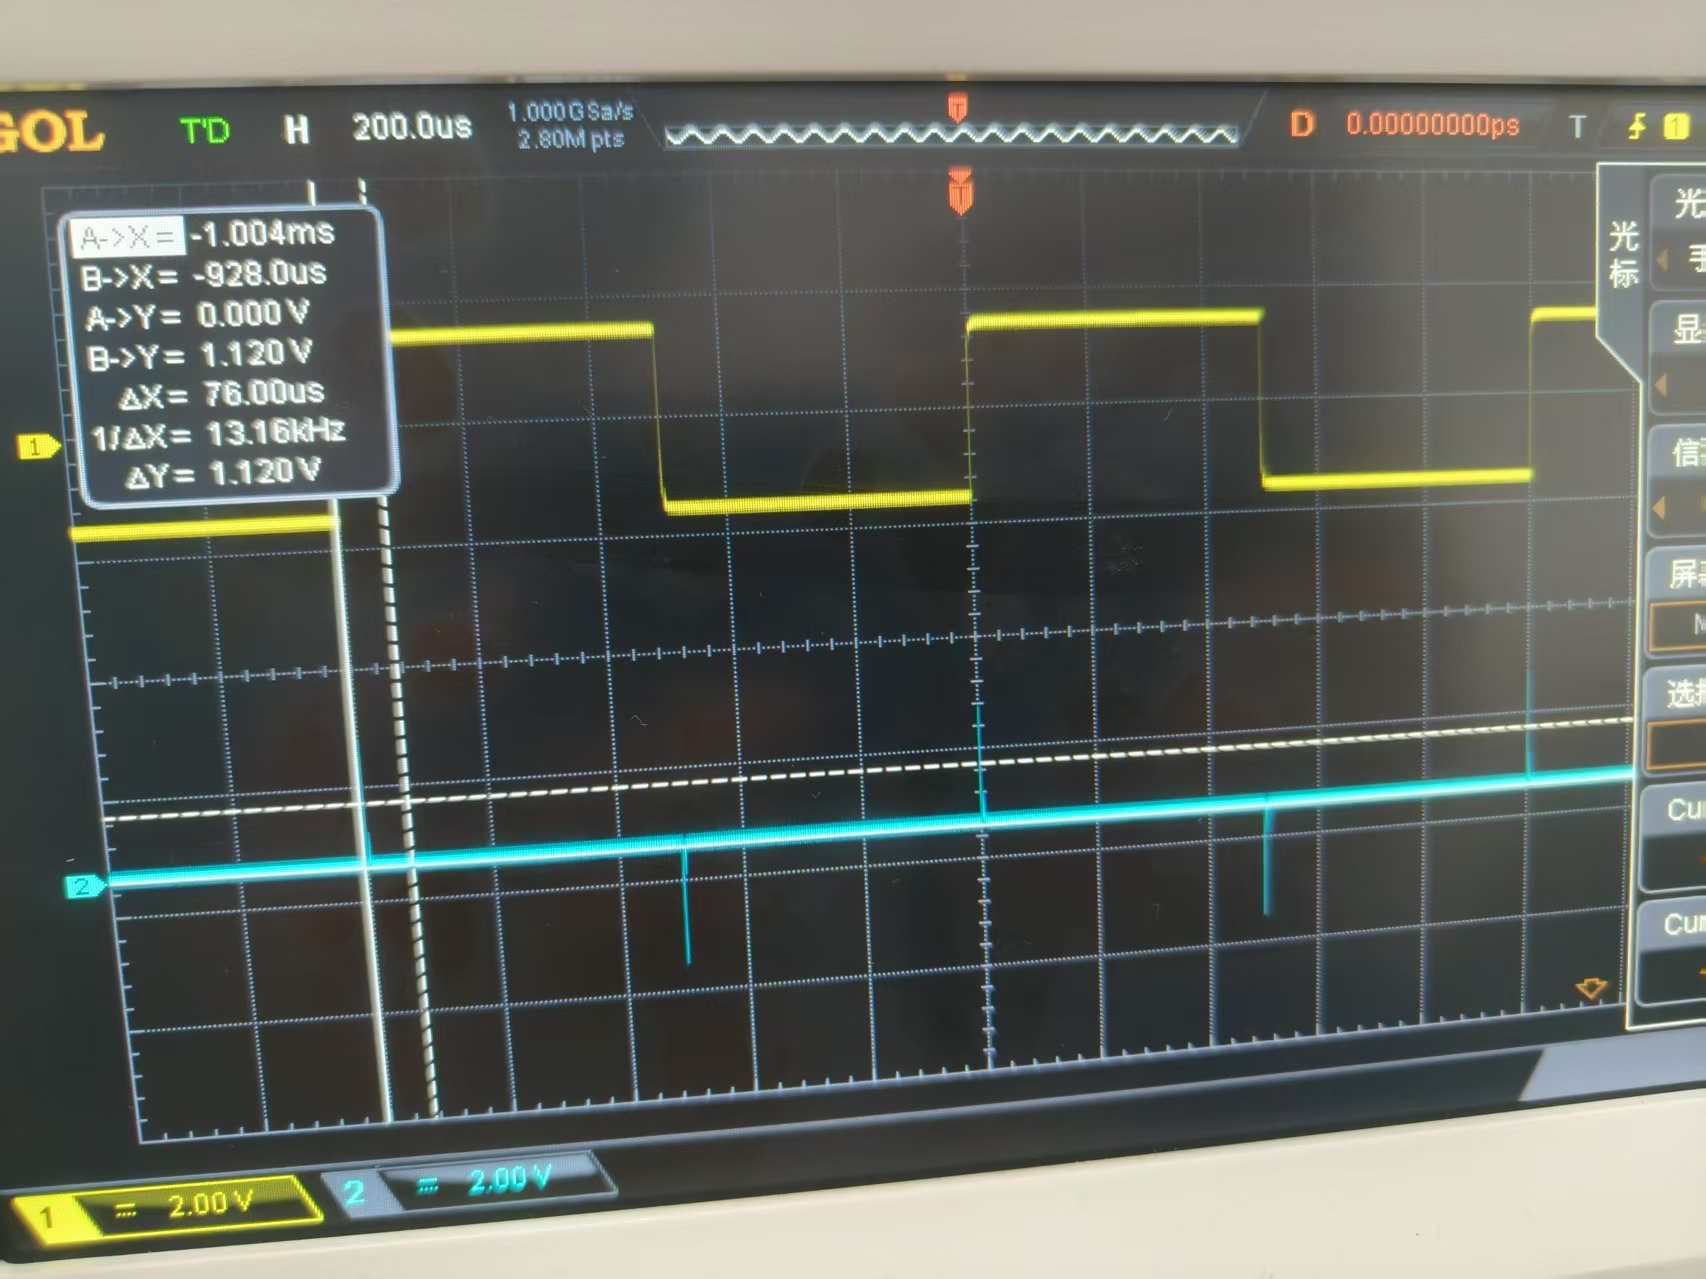
\includegraphics[width=0.35\textwidth]{100.jpg} \\
        (c) $\mathrm{R}=1k \Omega $ & (d) $\mathrm{R}=100 \Omega $ \\
    \end{tabular}
    \caption{微分电路$\mathrm{C}=0.01 \mu \mathrm{~F}$}
    \label{fig:grouped_images}
\end{figure}


\section{预习思考题}

1. 什么样的电信号可作为 RC 一阶电路零输入响应、零状态响应和完全响应的激励信号? 

阶跃信号可作为 RC 一阶电路零输入响应激励源

脉冲信号可作为 RC 一阶电路零状态响应激励源

正弦信号可作为 RC 一阶电路完全响应的激励源

2. 何谓积分电路和微分电路,它们必须具备什么条件?它们在方波序列脉冲的激励下,其
输出信号波形的变化规律如何?这两种电路有何作用?

1、积分电路定义:输出信号与输入信号的积分成正比的电路,应具备的条件:  $\tau=R C \gg t_p$

2、微分电路定义:输出电压与输入电压的变化率成正比的电路,应具备的条件: $\tau=R C \ll t_p$

3、输入信号波形的变化规律:

在方波序列脉冲的激励下,积分电路的输出信号波形在一定条件下成为三角波;而微分电路的输出信号波形为尖脉冲波。








\end{document}